\chapter{Fundamentaci�n Te�rica}

\label{chap:chapter1}

Escribir aqu� el cap�tulo 1. Ejemplo de acr�nimo es la \ac{UCI}. Esto es una cita de ejemplo \citep{Ou2013}. En la pr�xima oraci�n se muestra un ejemplo de un acr�nimo en ingl�s. Los sistemas de \ac{SCADA} son de gran importancia para la industria. 

\section{Secci�n de prueba de la \glsentrytext{UCI}} % example on how tu use glossaries or acronym in sections or another moving argument

Esto es una utilizaci�n de una palabra del glosario. El t�rmino \gls{Engine} es utilizado en \ul{este} ejemplo. Esta es una prueba de n�mero: $5.3$ donde se utiliza la coma autom�ticamente como separador.

Esto es una cita de ejemplo \citep{Alfadhlani2011,Mathew2010}.

\begin{figure}[!htb]
\centering
\captionbox{Vista del Arco de Moncloa\label{fig:DSC00461}}
{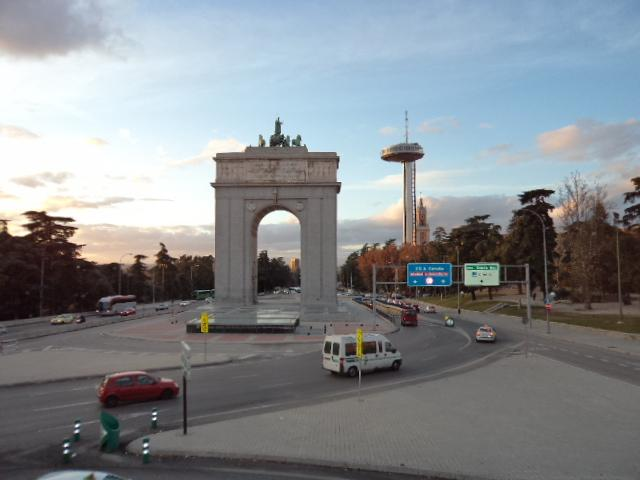
\includegraphics[width=0.7\linewidth]{Images/DSC00461}}
\end{figure}

En la Tabla \ref{Prueba} se observa \dots\\

\begin{table}[!h]
\centering
\captionbox{Caption de Prueba\label{Prueba}}
{
	\begin{tabular}{lllll}
	\hline \textbf{No. 1} & \textbf{No. 2} & \textbf{No. 3} & \textbf{No. 4} & \textbf{No. 5}\\ \hline
	12 & 12 & 56 & 56 &  56 \\ 
	12 & 12 & 56 & 56 &  56 \\
	\hline 
	\end{tabular}
}
\end{table}

\lipsum[1-50]
\begin{itemize}
\item Uno
\item Dos
\item Tres
\item Cuatro
\item Cinco
\end{itemize}

\lipsum[1-50]
\lipsum[1-50]
\lipsum[1-50]
\lipsum[1-50]
\lipsum[1-50]
\lipsum[1-50]